\chapter{ESPECIFICAÇÃO DO PROJETO} % (fold)
\label{cha:especificacao_do_projeto}

 O projeto consiste no desenvolvimento de um sistema de recomendação acoplado a uma rede social. As recomendações realizadas pelo sistema serão baseadas em similaridade de itens, em similaridade de perfil e na confiança implícita entre os usuários.

\section{Visão Geral do Sistema} % (fold)
\label{sec:visao_do_sistema}

O sistema de recomendação utilizará a rede social para obter as relações de amizade entre usuários. Esta relação é estabelecida entre dois usuários após ambos a confirmarem através do envio de um convite de amizade ou da aceitação deste.

Os usuários podem avaliar produtos (previamente cadastrados na base de dados) e receber recomendações de outras pessoas presentes na rede social. Tendo como base o comportamento dos usuários nestas atividades o sistema será capaz de enviar novas recomendações de produtos relevantes ao usuário.

 Os principais blocos do sistema podem ser vistos na Figura~\ref{fig:escopo}. A rede social é utilizada para o estabelecimento das relações de amizade, para a criação e visualização de avaliações dos produtos e para o envio de recomendações. O repositório é utilizado para armazenar os produtos cadastrados e as recomendações a serem enviadas. Já o sistema de recomendação tem o papel de analisar as informações contidas no repositório e gerar novas recomendações.

\begin{figure}
  \centering
  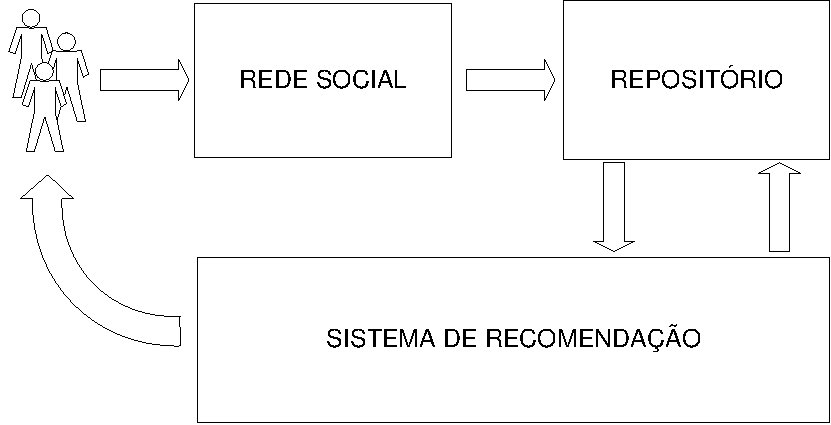
\includegraphics[width=\textwidth]{imagens/Diagrama_Visao_Geral}
  \caption{\it Diagrama de blocos do sistema}
  \label{fig:escopo}
\end{figure}

% section visao_do_sistema (end)

\section{Descrição do Sistema}

 Através do sistema os usuários poderão indicar o interesse em produtos e realizar recomendações a outros usuários. Quando um usuário avaliar um produto recomendado por outro o índice de confiança deste em relação ao outro é atualizado no sistema. Com base nas recomendações e nas avaliações o sistema irá inferir as seguintes informações:
 
\begin{itemize}

 \item Similaridade entre usuários

 \item Similaridade entre produtos

 \item Grau de confiança entre usuários

 \item Recomendações de produtos mais relevantes para um determinado usuário

\end{itemize}

 As recomendações geradas pelo sistema são baseadas nas avaliações de produtos feitas pelos usuários. A partir destas avaliações o sistema calcula a similaridade entre usuários, as relações de confiança e as relações encontradas entre os produtos.

\begin{figure}[htp]
 \centering
 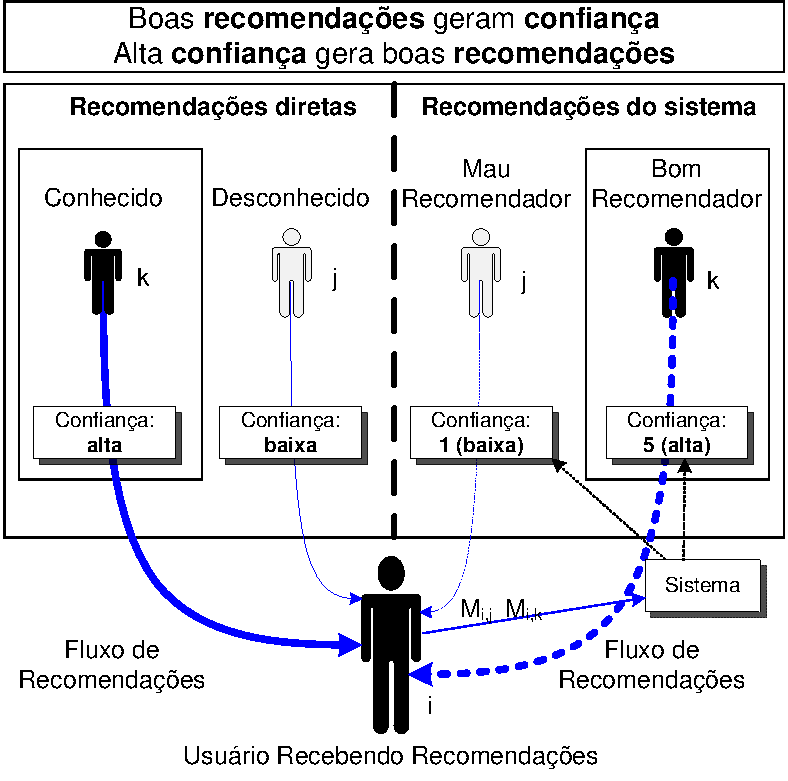
\includegraphics[width=\textwidth]{imagens/diagrama_confianca}
 \caption{\it Diagrama ilustrando o parâmetro de confiança na rede}
 \label{fig:diagrama_confianca}
\end{figure}
 
  O usuário do sistema tem a opção de buscar os produtos já cadastrados através de uma ferramenta de busca incorporada à rede social. Além disso, os usuários podem recomendar os produtos para outros usuários presentes na rede social. Os usuários são informados que devem sempre realizar boas recomendações. Uma boa recomendação é a indicação de um produto que o outro usuário provavelmente terá o máximo interesse.

 Ao receber uma recomendação o usuário tem a opção de a avaliar o produto e então o sistema atualiza as informações relativas aos seus interesses. As avaliações de produtos são feitas em uma escala de 1 a 5, onde 1 representa que o usuário não tem nenhum interesse no produto, e 5 significa que o usuário tem muito interesse no produto. Estas informações são utilizadas para verificar a similaridade entre usuários, a similaridade entre itens e o índice de confiança.
 
 Quando um usuário avalia um produto recomendado por outro, essa avaliação altera o grau de confiança do usuário que recomendou o produto em relação àquele que recebeu a recomendação. Caso a avaliação seja positiva, a confiança do receptor aumenta, porém, caso a avaliação seja negativa, significa que o usuário que recebeu a recomendação não a aceitou como relevante, diminuindo o grau de confiança.

 O parâmetro de confiança $C_{i,j}$, que representa a confiança que o usuário $i$ tem no usuário $j$, é calculado de acordo com a Equação~\ref{eq:param_trust}:
 
\begin{equation}
 C_{i,j} = \frac{M_{i,j} - 3}{2}
 \label{eq:param_trust} 
\end{equation}

 Onde
\begin{equation}
 M_{i,j} = \frac{{\sum_{i=0}^n}R_{i,j}}{n}
 \label{eq:media_notas}
\end{equation}

 Sendo que $M_{i,j}$ é a média das notas que o usuário $i$ deu aos produtos recomendados pelo usuário $j$ e $n$ o número de recomendações que $i$ recebeu de $j$. Para o parâmetro de confiança $C_{i,j}$ ficar normalizado na escala [-1,1], assim como os parâmetros de similaridade entre perfis e itens, a Equação~\ref{eq:param_trust} é aplicada.

 Desse modo, o parâmetro de confiança é a média das notas dadas aos produtos recomendados normalizada na escala [-1,1]. A Figura~\ref{fig:diagrama_confianca} ilustra as relações entre os usuários da rede social e os parâmetros de confiança calculados.
 
 O algoritmo RBC leva em conta que as pessoas que fazem boas recomendações têm um alto grau de confiança do usuário que recebeu as indicações de produtos. No plano social, a hipótese é que o bom recomendador é uma pessoa conhecida, enquanto os desconhecidos são mau recomendadores. Assim, o bom recomendador possui um alto grau de confiança, permitindo ao sistema que o fluxo de recomendações entre pessoas confiáveis seja maior do que entre as não confiáveis.
 
 O sistema também recomenda produtos utilizando os algoritmos RBP e RBI, que também levam em conta as avaliações de produtos feitas pelos usuários no sistema. Com relação ao RBC, o RBP e o RBI utilizam todas as avaliações de produtos feitas na rede e o RBC utiliza apenas as avaliações de produtos recomendados ao usuário alvo.
 
 Todas as informações sobre as avaliações são armazenadas no repositório para que o sistema de recomendação as consulte e seja capaz de realizar recomendações de outros produtos aos usuários. Esse é um dos propósitos do sistema de recomendação: mostrar ao usuário apenas informações relevantes. A Figura~\ref{fig:aspectos_funcionais} apresenta os diagrama de blocos dos aspectos do sistema e a relação entre eles.
 
\begin{figure}
 \centering
 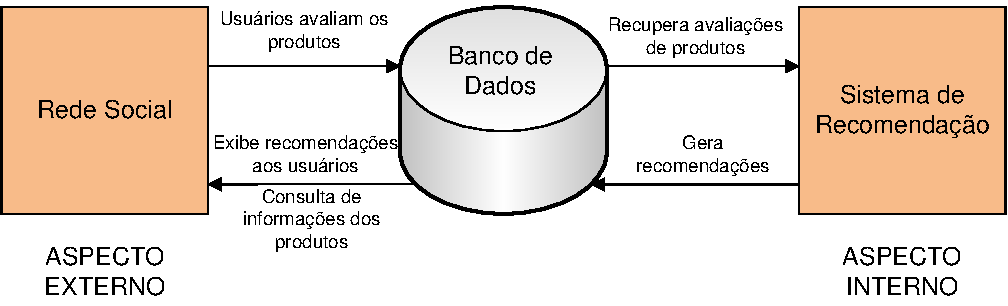
\includegraphics[width=\textwidth]{imagens/Implementacao_Detalhe2}
 \caption{\it Aspectos funcionais do sistema}
 \label{fig:aspectos_funcionais}
\end{figure}

\section{Funcionalidades principais} % (fold)
\label{sec:funcionalidades_principais}

Abaixo estão sumarizadas as principais funcionalidades do sistema acompanhadas das descrições em formato de \textit{user stories}\cite{557458}:

\begin{itemize}
  
  \item Envio de convite
  \subitem Como usuário, quero convidar outra pessoa a ingressar na rede social para que ela possa utilizar o sistema.
  
  \item Pedido de amizade
  \subitem Como usuário, quero convidar outro usuário a estabelecer uma relação de amizada na rede para que eu possa acompanhar as atividades dele na rede.
  
  \item Confirmação de amizade
  \subitem Como usuário, quero confirmar ou rejeitar um pedido de amizade para que eu possa acompanhar as atividades dos meus amigos pelo sistema.
	
	\item Avaliação de produto
  \subitem Como usuário, quero fazer a minha avaliação de produtos para que outros tenham conhecimento da minha opinião.
  
	\item Envio de recomendação de produto a outro usuário
  \subitem Como recomendador, quero enviar uma recomendação de produto para outra pessoa para que ela conheça a minha opinião sobre este item.
  
	\item Recomendação de produtos
	\subitem Como usuário, eu quero receber uma lista de produtos que eu provavelemente goste para que eu não precise filtrar os itens que me interessam.

    \item Visualização das avaliações dos usuários
    \subitem Como usuário, quero estar ciente sobre as últimas avaliações dos meus amigos para que eu possa saber o que acontece no meu contexto social e conheça novos produtos.
	
\end{itemize}

\section{Requisitos não-funcionais}

Os principais requisitos não-funcionais do sistema são:

\begin{itemize}

    \item Interface web compatível as últimas versões dos \textit{browsers} Internet Explorer, Mozilla Firefox e Safari.
    
    \item \textit{Backend} compatível com servidores Linux.

    \item Tempo médio de resposta menor que 2 segundos para 10 usuários simultâneos quando executado em um servidor com processador Intel Core 2 Duo T7250 ou superior e 2 GB de memória RAM. % esta é a configuração do meu notebook -- Allan

\end{itemize}

\section{Limites do Sistema}

\begin{itemize}
  
    \item O sistema não faz processamento de linguagem natural\footnote{\textit{Natural Language Processing (NLP)}}

\end{itemize}

\section{Implementação} % (fold)
\label{sec:implementacao}

A principal linguagem de programação utilizada no projeto foi Ruby, uma linguagem de script, com tipagem dinâmica, forte e implícita. Além disso, o Ruby permite uma abordagem multi-paradigma bem equilibrada entre os paradigmas orientado a objetos, funcional, imperativo e reflexivo. 

O \emph{framework} web Ruby on Rails foi escolhido para implementação do projeto. O Rails permite a adição de novas funcionalidades de forma ágil, pois é baseado em uma arquitetura \emph{Model-View-Controller}\cite{burbeck1992applications} (MVC) e segue os princípios \emph{Convention over Configuration}\cite{ruby2009agile} (CoC) e \emph{Don't Repeat Yourself}\cite{hunt-don} (DRY).

A lingugem Python também foi utilizada no projeto para algumas tarefas secundárias. Um script foi escrito nesta linguagem para fazer um \emph{crawler} e o \emph{parsing} de cerca de vinte mil produtos do site Submarino\footnote{www.submarino.com} para preencher a base de dados de produtos.

O SQLite é uma biblioteca independente que implementa um banco de dados SQL transacional, sem a necessidade de configurações. Este foi o gerenciador de banco de dados escolhido para o projeto, pois ele atende aos requistos de performance e facilita geração de backups.

Visando permitir um padrão de usabilidade aceitável para o usuário comum, algumas interações no sistema são realizadas via AJAX (Asynchronous JavaScript And XML). Através dessa técnica a aplicação pode obter dados do servidor de forma assíncrona sem interferir na apresentação e no comportamento da página atual. Esse recurso foi utilizado para permitir que os usuários registrassem o interesse em produtos sem que a página fosse totalmente recarregada. Como o uso dessa técnica requer utilização de JavaScript no \emph{browser} (cliente), e nem todos os \emph{browsers} tem JavaScript habilitado, o sistema tolera esse deficiência do cliente e possibilita neste caso o acesso através de uma requisição síncrona com recarregamento total da página.

A Figura~\ref{fig:rater-ajax} apresentar o painel de avaliação de produto que utiliza a técnica de AJAX. Ao clicar em uma das estrelas, uma requisição é enviada ao servidor para o cadastro da avaliação e, em caso de sucesso, a resposta enviada de volta ao \emph{browser} atualiza o estilo do elemento selecionado, indicando que a avaliação foi realizada.
\begin{figure}
 \centering
 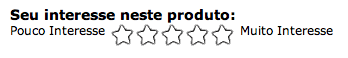
\includegraphics{imagens/rater-ajax}
 \caption{\it Avaliação de produto via AJAX}
 \label{fig:rater-ajax}
\end{figure}

O sistema conta com uma interface de administração na qual é possível enviar convites para novos usuários se integrarem a rede social. Quando um novo convite é gerado, automaticamente um \emph{token} pseudo-aletório é associado a ele. Esse \emph{token} é enviado através de e-mail, permitindo o registro apenas do convidado associado ao convite. A autenticação do usuário é feita através de login com e-mail e senha. O \emph{framework} escolhido para prover os mecanismos de autenticação foi o Warden\footnote{http://github.com/hassox/warden}, pois ele é adequado para oferecer poderosas opções de autenticação e pode ser utilizado em aplicações Rails através do Rack\footnote{http://rack.rubyforge.org/}.

A arquitetura cliente/servidor em três camadas, apresentada na Figura~\ref{fig:three_tier}, foi adotada na implementação do projeto. Essa escolha possibilita a modificação ou substituição de uma das camadas sem afetar as demais. Além disso, a separção entre as camadas de aplicação e de dados facilita o balanceamento da carga do sistema. Por fim, as políticas de segurança aplicadas no servidor podem ser rigorosas e, mesmo assim, não incomodar excessivamente os clientes.

\begin{figure}
 \centering
 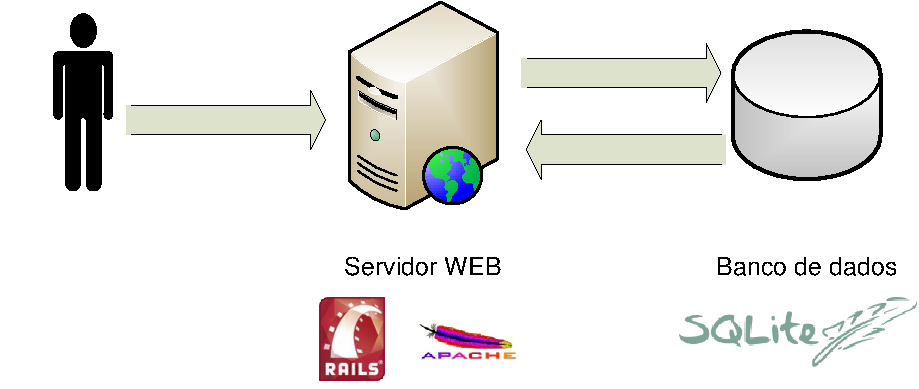
\includegraphics[width=\textwidth]{imagens/Implementacao_Detalhe}
 \caption{\it Arquitetura em três camadas}
 \label{fig:three_tier}
\end{figure}

% section implementacao (end)

% chapter especificacao_do_projeto (end)
